% =====================================================================
%  Apostila — reúne o conteudo.tex de todas as aulas num só PDF.
%  Para incluir/excluir uma aula, comente a linha correspondente.
% =====================================================================
\documentclass[apostila]{tmlnotas}

\graphicspath{
  {../aulas/01-o-que-e-ml/figs/}
  {../aulas/02-python-numpy-jax/figs/}
  {../aulas/03-treino-teste-validacao/figs/}
  {../aulas/04-gradiente-descendente/figs/}
  {../aulas/05-arvores-redes/figs/}
  {../aulas/06-casos-economia/figs/}
}

\begin{document}
\capaapostila
\tableofcontents

% =====================================================================
%  Aula 1 — conteúdo das notas (incluído por notas.tex e pela apostila)
% =====================================================================
\aula{1}{O que é Aprendizado de Máquina?}[O que é ML?]

\begin{intuicao}[title={Objetivos da aula}]
Ao final desta aula você deve ser capaz de: (i) explicar o que significa um
algoritmo ``aprender'' e por que o desempenho é medido em casos novos;
(ii) distinguir problemas de previsão ($\hat y$) de problemas de inferência
($\hat\beta$); (iii) classificar uma tarefa como regressão, classificação ou
agrupamento; (iv) formular um problema econômico como tarefa de aprendizado de
máquina; e (v) reconhecer o fluxo básico de um projeto em \pkg{scikit-learn}.
\end{intuicao}

\section{Três perguntas}

Comecemos por três perguntas que um economista poderia receber numa mesma
semana. Quanto deve valer um apartamento de 70\,m² em Pinheiros? Um cliente que
pede um empréstimo vai pagá-lo? Que ``tipos'' de famílias existem nos dados de
uma pesquisa de orçamentos domésticos?

As três têm algo em comum: podem ser respondidas olhando para \emph{muitos casos
parecidos} e extraindo deles um padrão. Ninguém escreve à mão a regra que liga
área e localização ao preço; a regra é \emph{aprendida} a partir de transações
passadas. Mas as três também diferem no que queremos obter: na primeira, um
número; na segunda, uma categoria (paga ou não paga); na terceira, grupos que
ninguém rotulou antes. Essas diferenças dão nome aos principais tipos de
aprendizado de máquina, e reconhecê-las é o primeiro passo de qualquer projeto.

\section{O que significa ``aprender''?}

\begin{definicao}
Um programa \emph{aprende} com a experiência $E$, em relação a uma classe de
tarefas $T$ e a uma medida de desempenho $P$, se o seu desempenho nas tarefas
em $T$, medido por $P$, melhora com a experiência $E$ \parencite{mitchell1997}.
\end{definicao}

A definição é deliberadamente operacional: não fala de ``inteligência'', fala de
desempenho mensurável. No exemplo do crédito, a tarefa $T$ é prever se um novo
cliente ficará inadimplente; a experiência $E$ é o histórico de clientes passados,
com a informação de quem pagou; e o desempenho $P$ pode ser a proporção de
clientes \emph{novos} classificados corretamente.

A palavra \emph{novos} é o coração da definição. Um programa que simplesmente
guardasse a lista de clientes passados acertaria 100\% deles, e não teria
aprendido nada útil, porque o banco precisa decidir sobre quem ainda não está na
lista. Aprender é \emph{generalizar}; decorar não é aprender. A Aula 3 inteira
será dedicada a medir essa diferença com honestidade.

\subsection{A mesma ideia em linguagem econométrica}

Formalmente, supomos que o alvo $y$ e os atributos $\vx$ estão ligados por
\begin{equation}\label{eq:a02-modelo}
  y = f(\vx) + \varepsilon,
\end{equation}
em que $f$ é desconhecida e $\varepsilon$ reúne tudo o que $\vx$ não explica.
Dispomos de um conjunto de dados $\data = \{(\vx_i, y_i)\}_{i=1}^{n}$.
\emph{Aprender} é usar $\data$ para construir uma aproximação $\hf$;
\emph{usar o modelo} é calcular $\hat y = \hf(\vx_{\text{novo}})$ para casos
que não estavam em $\data$.

\begin{conexao}
Se impomos $f(\vx) = \vx\T\vbeta$ e escolhemos $\hvbeta$ minimizando a soma
dos quadrados dos resíduos, \cref{eq:a02-modelo} é o modelo de regressão linear
e o MQO é o algoritmo de aprendizado. Não há ruptura entre econometria e
aprendizado de máquina: há uma mudança de \emph{ênfase}, como veremos a seguir.
\end{conexao}

\subsection{Um pequeno dicionário}

As duas comunidades desenvolveram vocabulários próprios para as mesmas ideias.
A \cref{tab:a02-dicionario} reúne as traduções mais comuns; vale guardá-la, porque
a documentação das bibliotecas usa sempre o vocabulário da direita.

\begin{table}[ht]
  \centering\small
  \caption{Termos equivalentes em econometria e aprendizado de máquina.}
  \label{tab:a02-dicionario}
  \begin{tabular}{@{}lll@{}}
    \toprule
    Econometria & Aprendizado de máquina & Símbolo \\
    \midrule
    variável dependente      & alvo, rótulo (\emph{target}, \emph{label}) & $y$ \\
    variáveis explicativas   & atributos (\emph{features})                  & $\vx$ \\
    observação               & exemplo, instância                           & $(\vx_i,y_i)$ \\
    amostra                  & conjunto de treino                           & $\dtreino$ \\
    estimar                  & treinar, ajustar (\emph{fit})                & $\data\mapsto\hf$ \\
    parâmetros               & pesos (\emph{weights})                       & $\vbeta$, $\vw$ \\
    intercepto               & viés (\emph{bias})                           & $\beta_0$, $b$ \\
    valor ajustado           & previsão (\emph{prediction})                 & $\hat y$ \\
    \bottomrule
  \end{tabular}
\end{table}

\begin{atencao}
Em ML, ``viés'' (\emph{bias}) pode designar simplesmente o intercepto de um
modelo, sem relação com o viés de um estimador ($\E[\hat\theta]-\theta$). O
contexto decide. Na Aula 3 encontraremos o viés no segundo sentido, no
compromisso entre viés e variância.
\end{atencao}

\section{Estatística, econometria e aprendizado de máquina}

\subsection{Duas culturas}

\textcite{breiman2001cultures} descreveu duas culturas na análise de dados
(\cref{fig:a02-culturas}). Na \emph{cultura da modelagem de dados}, dominante
na estatística e na econometria, o pesquisador especifica um modelo para o
processo gerador dos dados (por exemplo, $y=\mX\vbeta+\ve$ com hipóteses sobre
$\ve$) e o interesse recai sobre os parâmetros: seus valores, seus erros-padrão,
sua interpretação. Na \emph{cultura algorítmica}, o processo gerador é tratado
como uma caixa-preta; escolhe-se o algoritmo que melhor prevê casos novos, e a
validação fora da amostra é o critério de qualidade.

\begin{figure}[ht]
  \centering
  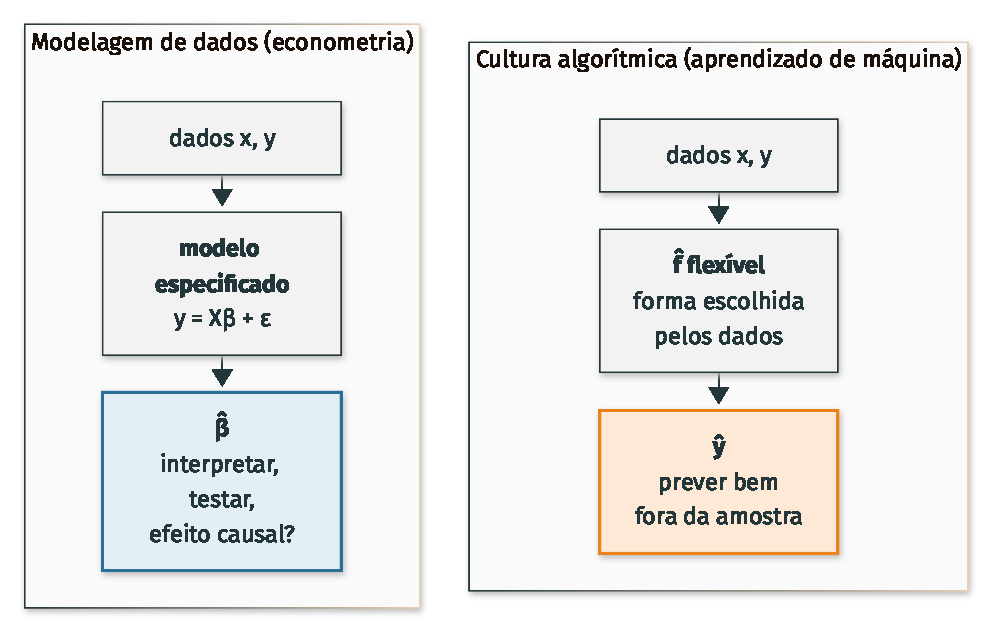
\includegraphics[width=0.78\linewidth]{a01_duas_culturas}
  \caption{As duas culturas de \textcite{breiman2001cultures}. O que muda não é a
  matemática disponível, e sim o produto final que se deseja: $\hat\beta$ ou $\hat y$.}
  \label{fig:a02-culturas}
\end{figure}

\subsection{Problemas de \texorpdfstring{$\hat\beta$}{beta} e problemas de \texorpdfstring{$\hat y$}{y}}

\textcite{mullainathan2017} traduzem essa distinção para a economia aplicada.
Muitos trabalhos empíricos são \emph{problemas de $\hat\beta$}: qual o efeito de
um ano adicional de estudo sobre o salário? Um programa de transferência de renda
afeta a frequência escolar? Aqui o objetivo é entender um mecanismo, e a
dificuldade central é a \emph{identificação}: saber o que aconteceria se
mudássemos $x$, mantido o resto constante. Outros são \emph{problemas de
$\hat y$}: qual a probabilidade de um cliente ficar inadimplente? Qual será a
inflação do próximo mês? Aqui importa acertar casos ainda não observados, e a
dificuldade central é a \emph{generalização}.

O aprendizado de máquina foi construído para problemas de $\hat y$. Usá-lo para
responder perguntas de $\hat\beta$ sem cuidados adicionais é um erro comum, e
a \cref{fig:a02-prever} mostra por quê.

\begin{figure}[ht]
  \centering
  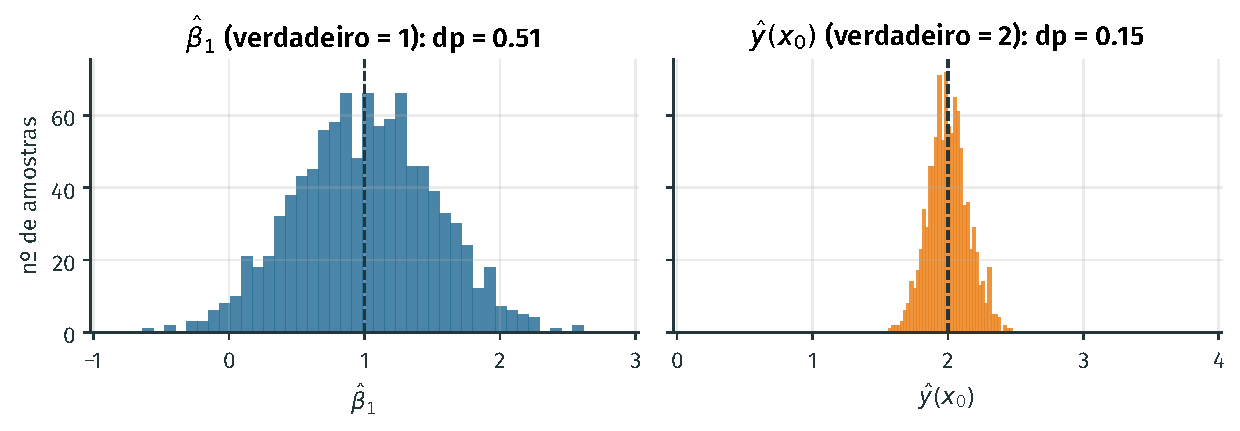
\includegraphics[width=0.85\linewidth]{a01_prever_inferir}
  \caption{Mil amostras de $n=100$ observações de $y = x_1 + x_2 + \varepsilon$,
  com $\operatorname{corr}(x_1,x_2)=0{,}98$. Em cada amostra estimamos o modelo por
  MQO. O coeficiente de $x_1$ varia muito entre amostras; a previsão no ponto
  $x_0 = (1,1)$ varia bem menos.}
  \label{fig:a02-prever}
\end{figure}

\begin{intuicao}
Quando $x_1$ e $x_2$ andam juntos, os dados informam bem o efeito
\emph{conjunto} $\beta_1+\beta_2$, que é o que a previsão em $x_0=(1,1)$ usa,
mas informam mal como esse efeito se divide entre $\beta_1$ e $\beta_2$.
Para prever, a divisão não importa; para interpretar, ela é tudo. Por isso um
modelo com ótimo desempenho preditivo pode ter coeficientes que mudam de sinal
de uma amostra para outra.
\end{intuicao}

\subsection{Guarda-chuva ou dança da chuva?}

\textcite{kleinberg2015} propõem uma imagem simples. Quem decide se leva o
guarda-chuva só precisa \emph{prever} se vai chover; o motivo da chuva é
irrelevante. Quem decide se faz a dança da chuva precisa saber se a dança
\emph{causa} chuva; nenhuma previsão responde a isso. Os autores mostram que
muitas decisões de política pública são do primeiro tipo, ou seja,
\emph{problemas de política preditiva}. Um exemplo do artigo: identificar
pacientes idosos que provavelmente morreriam no ano seguinte, para os quais
uma cirurgia de prótese de quadril traria pouco benefício. A decisão depende de
uma previsão, não de um efeito causal.

\begin{conexao}
Previsão e causalidade não são rivais. Métodos modernos de inferência causal
usam aprendizado de máquina em etapas puramente preditivas, por exemplo para
controlar de forma flexível muitas variáveis de confusão
\parencite{chernozhukov2018,athey2019}. Voltaremos a isso na Aula 6.
\end{conexao}

\section{Tipos de aprendizado}

A pergunta que organiza a taxonomia é: \emph{observamos o alvo $y$?}
(\cref{fig:a02-taxonomia}).

\begin{figure}[ht]
  \centering
  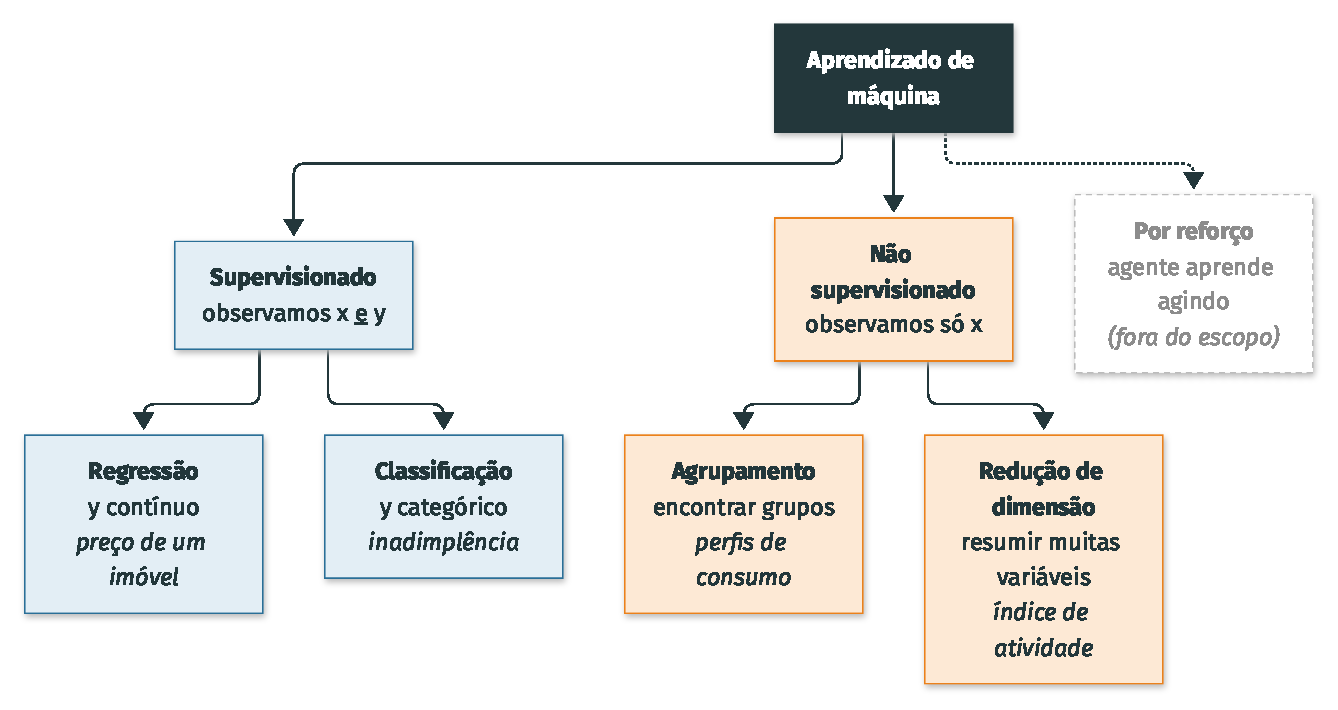
\includegraphics[width=0.82\linewidth]{a01_taxonomia}
  \caption{Tipos de aprendizado de máquina. Neste curso tratamos dos ramos
  supervisionados; o aprendizado por reforço fica fora do escopo.}
  \label{fig:a02-taxonomia}
\end{figure}

\begin{description}
  \item[Aprendizado supervisionado.] Observamos pares $(\vx_i, y_i)$: os dados
  ``supervisionam'' o algoritmo com respostas corretas. Se $y$ é contínuo
  (preço, salário, inflação), temos uma tarefa de \emph{regressão}; se $y$ é
  categórico (inadimplente ou não, setor de atividade), uma tarefa de
  \emph{classificação}.
  \item[Aprendizado não supervisionado.] Observamos apenas $\vx_i$. O objetivo é
  descobrir estrutura: grupos de observações parecidas (\emph{agrupamento}) ou
  poucas combinações de variáveis que resumem muitas (\emph{redução de
  dimensionalidade}, como num índice de condições financeiras construído a
  partir de dezenas de séries).
  \item[Aprendizado por reforço.] Um agente aprende a agir por tentativa e erro,
  recebendo recompensas do ambiente. É uma área ativa em economia computacional,
  mas exige ferramentas que estão além deste curso.
\end{description}

A \cref{fig:a02-tarefas} ilustra as três tarefas principais. Note a diferença
no terceiro painel: não há cores ``verdadeiras''. O algoritmo propõe três grupos
porque nós pedimos três; se pedíssemos cinco, ele proporia cinco. Interpretar e
validar os grupos é responsabilidade do analista.

\begin{figure}[ht]
  \centering
  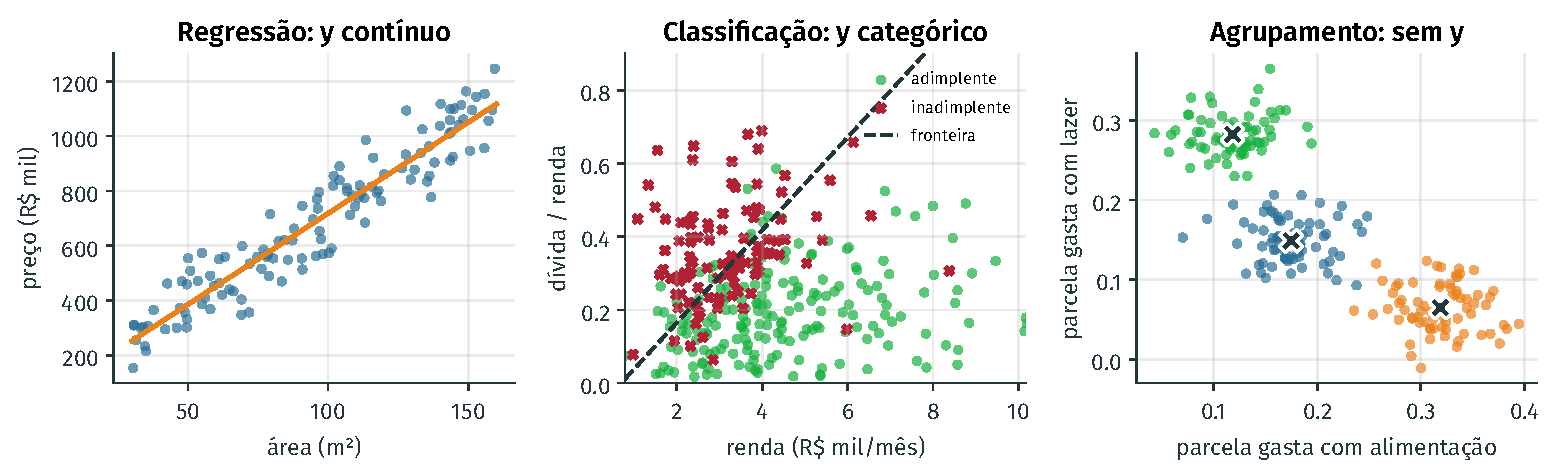
\includegraphics[width=\linewidth]{a01_tarefas}
  \caption{Regressão (prever um número), classificação (prever uma categoria,
  com a fronteira de decisão tracejada) e agrupamento (propor grupos sem rótulos;
  os X marcam os centros encontrados pelo algoritmo $k$-médias). Dados simulados.}
  \label{fig:a02-tarefas}
\end{figure}

\subsection{Formular é escolher}

A tarefa não está escrita nos dados; é uma escolha do analista. Com a mesma
base de domicílios, podemos prever a renda em reais (regressão), prever se a
renda supera dois salários mínimos (classificação) ou procurar perfis de
domicílios sem alvo nenhum (agrupamento). Discretizar um alvo contínuo
simplifica a comunicação, mas descarta informação. O critério para escolher
é a \emph{decisão} que a previsão vai apoiar.

\section{Formulando problemas econômicos}

Antes de abrir o Python, vale preencher uma ficha com seis itens:

\begin{enumerate}[label=\arabic*.]
  \item \textbf{Decisão}: quem vai usar a previsão, e para quê?
  \item \textbf{Unidade de observação}: o que é uma linha da base?
  \item \textbf{Alvo $y$}: o que exatamente queremos prever, com definição precisa?
  \item \textbf{Atributos $\vx$}: que informação está disponível \emph{no momento
        em que a decisão é tomada}?
  \item \textbf{Tarefa}: regressão, classificação ou agrupamento?
  \item \textbf{Métrica}: como saberemos se o modelo é bom o suficiente para a decisão?
\end{enumerate}

\begin{exemplo}[title={Exemplo: crédito pessoal}]
\textbf{Decisão:} aprovar ou recusar um pedido de empréstimo.
\textbf{Unidade:} um pedido.
\textbf{Alvo:} atraso superior a 90 dias nos 12 meses seguintes (sim/não).
\textbf{Atributos:} renda declarada, idade, razão dívida/renda, histórico no
cadastro positivo, todos conhecidos na data do pedido.
\textbf{Tarefa:} classificação.
\textbf{Métrica:} os dois erros têm custos diferentes. Recusar um bom pagador
custa a margem do empréstimo; aprovar um mau pagador custa o principal. A
métrica deve refletir essa assimetria (Aula 3).
\end{exemplo}

\begin{atencao}
O item 4 é onde a maioria dos projetos tropeça. Se um atributo só é conhecido
\emph{depois} do evento que queremos prever (``número de cartas de cobrança
enviadas'' para prever inadimplência, ou a revisão final do PIB para prever o
próprio PIB), o modelo parecerá excelente nos dados históricos e será inútil na
prática. Esse fenômeno, o \emph{vazamento de dados}, é um dos temas da Aula 3.
\end{atencao}

\section{Fluxo de trabalho em Python}

Um projeto de aprendizado supervisionado segue, em linhas gerais, o fluxo da
\cref{fig:a02-fluxo}. As etapas em laranja (separar e avaliar) são o assunto da
Aula 3; a etapa em azul (treinar) será aberta por dentro nas Aulas 4 e 5.

\begin{figure}[ht]
  \centering
  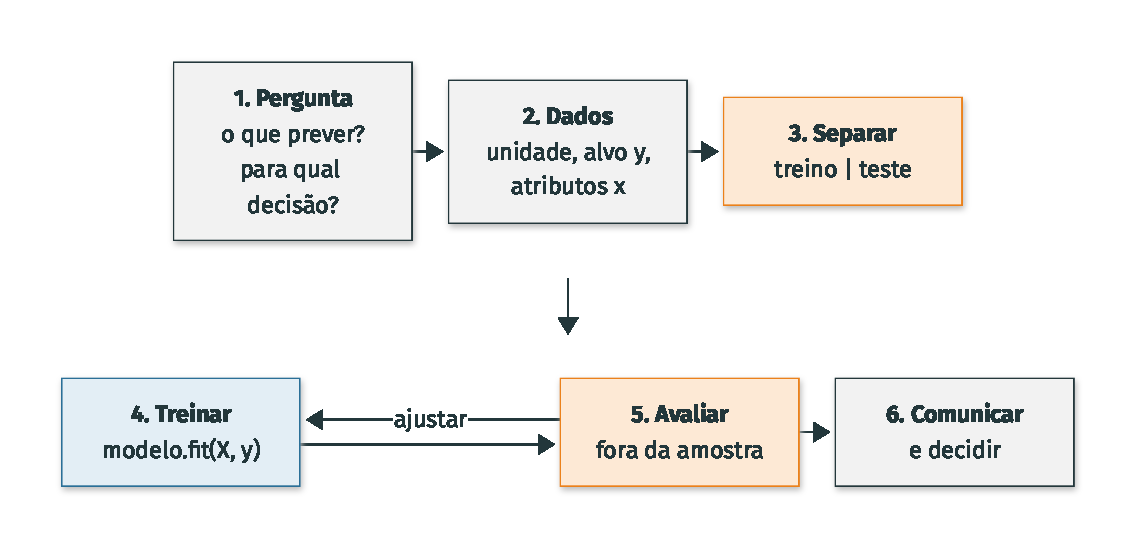
\includegraphics[width=\linewidth]{a01_fluxo}
  \caption{Fluxo de um projeto de aprendizado supervisionado. O ciclo
  avaliar–ajustar pode se repetir várias vezes, mas sempre com dados de
  validação; o conjunto de teste é usado uma única vez, no final.}
  \label{fig:a02-fluxo}
\end{figure}

A biblioteca \pkg{scikit-learn} \parencite{pedregosa2011} padroniza esse fluxo:
todo modelo é um objeto com os métodos \py{fit} (aprender) e \py{predict}
(prever).

\begin{codigo}
from sklearn.model_selection import train_test_split
from sklearn.linear_model import LinearRegression
from sklearn.dummy import DummyRegressor
from sklearn.metrics import mean_squared_error

X_tr, X_te, y_tr, y_te = train_test_split(X, y, test_size=0.2, random_state=0)

for modelo in [DummyRegressor(strategy="mean"), LinearRegression()]:
    modelo.fit(X_tr, y_tr)
    rmse = mean_squared_error(y_te, modelo.predict(X_te)) ** 0.5
    print(type(modelo).__name__, round(rmse, 3))
\end{codigo}

Dois detalhes merecem destaque. Primeiro, o desempenho é calculado em
\py{X_te}, \py{y_te}, dados que o modelo não viu durante o \py{fit}.
Segundo, o laço compara o modelo com uma \emph{referência ingênua}, que prevê
sempre a média do treino.

\begin{atencao}
Um número de desempenho isolado não diz nada. Se 95\% dos clientes pagam em
dia, um ``modelo'' que declara que \emph{todos} pagam acerta 95\% dos casos e
não tem nenhuma utilidade. Compare sempre com uma referência ingênua: a média
(regressão), a classe mais frequente (classificação) ou o último valor
observado (séries temporais).
\end{atencao}

\section{Resumo e leituras}

\begin{itemize}[nosep]
  \item Aprender é melhorar o desempenho em \emph{casos novos} com a experiência.
  \item A regressão linear já é um algoritmo de aprendizado; o que muda no ML é a
        ênfase em $\hat y$ e na validação fora da amostra.
  \item Bons $\hat y$ não garantem $\hat\beta$ interpretáveis.
  \item Supervisionado (regressão, classificação) versus não supervisionado
        (agrupamento, redução de dimensão).
  \item Formular vem antes de modelar; os atributos precisam estar disponíveis no
        momento da decisão.
  \item \py{fit}, \py{predict} e uma referência ingênua, sempre.
\end{itemize}

\noindent\textbf{Leituras sugeridas.} \textcite{mullainathan2017} é a melhor
porta de entrada para economistas. \textcite[cap.~2]{james2021} apresenta a
formulação estatística com exemplos acessíveis. \textcite{breiman2001cultures}
e os comentários publicados junto ao artigo continuam atuais. Para um panorama
das aplicações em economia, \textcite{athey2019} e \textcite{varian2014}.

% =====================================================================
%  Aula 2 — conteúdo das notas (incluído por notas.tex e pela apostila)
%  Figuras: use apenas o nome (a02_...), o graphicspath resolve.
% =====================================================================
\aula{2}{Computação aplicada: de Python ao aprendizado de máquina}[Computação aplicada]

\begin{intuicao}[title={Objetivos da aula}]
Ao final desta aula você deve ser capaz de: (i) escrever pequenos programas em
Python com variáveis, listas, dicionários, condicionais, laços e funções;
(ii) usar o \pkg{NumPy} para fazer contas com vetores e matrizes inteiros,
inclusive o MQO; (iii) ler, filtrar, agrupar e resumir uma base de dados com o
\pkg{pandas}; (iv) explicar por que, com sorteio, a diferença de médias estima
o efeito de um programa, e por que um grupo de comparação inadequado produz
viés; (v) treinar um modelo por gradiente descendente com o \pkg{JAX}; e
(vi) usar o roteiro \py{fit}/\py{predict} do \pkg{scikit-learn}.
\end{intuicao}

\section{A pergunta: o programa funcionou?}

Imagine que você trabalha numa secretaria de trabalho e precisa avaliar um
programa de qualificação: as pessoas que passaram por ele ganham mais do que
ganhariam sem ele? A pergunta é simples de formular e difícil de responder,
porque nunca observamos a mesma pessoa nas duas situações. Esta aula responde a
uma pergunta desse tipo com dados reais e, no caminho, constrói a caixa de
ferramentas computacional que usaremos no resto do curso.

A escolha de aprender as ferramentas resolvendo um problema não é acidental.
Fluência em programação vem de usar a linguagem para fazer algo que importa, e
não de decorar comandos. Por isso cada ferramenta entra no momento em que
precisamos dela: Python para organizar alguns casos, \pkg{NumPy} para fazer as
contas sobre todos, \pkg{pandas} para ler e resumir a base, \pkg{JAX} para
treinar um modelo e \pkg{scikit-learn} para usar modelos prontos.

\section{O experimento NSW e a pergunta de LaLonde}

O \emph{National Supported Work Demonstration} (NSW) foi um programa americano
dos anos 1970 que oferecia emprego subsidiado e acompanhamento a pessoas com
muita dificuldade de entrar no mercado de trabalho. O detalhe que o tornou
famoso entre economistas é que as vagas foram \emph{sorteadas} entre os
candidatos: os sorteados formam o grupo de \emph{tratados}; os não sorteados,
o grupo de \emph{controle}.

\textcite{lalonde1986} usou o experimento como gabarito. Primeiro, o sorteio dá
o efeito do programa. Depois, finge-se que não houve sorteio: os controles são
trocados por pessoas de pesquisas domiciliares (a CPS e o PSID) e aplicam-se os
métodos econométricos da época. A conclusão, em geral desanimadora, foi que
esses métodos frequentemente se afastavam muito do gabarito, e o artigo se
tornou uma referência na avaliação de políticas. Usamos a subamostra de homens
de \textcite{dehejia1999}, que mantém quem tem a renda de 1974 informada: 185
tratados e 260 controles, além de 15.992 homens da CPS. As variáveis estão na
\cref{tab:a02-variaveis}.

\begin{table}[ht]
  \centering\small
  \caption{Variáveis da base NSW (subamostra de Dehejia e Wahba).}
  \label{tab:a02-variaveis}
  \begin{tabular}{@{}ll@{}}
    \toprule
    Variável & Significado \\
    \midrule
    \texttt{treat} & 1 se foi sorteado para o programa \\
    \texttt{age}, \texttt{education} & idade e anos de estudo \\
    \texttt{black}, \texttt{hispanic}, \texttt{married} & \emph{dummies} de raça/etnia e estado civil \\
    \texttt{nodegree} & 1 se não concluiu o ensino médio \\
    \texttt{re74}, \texttt{re75} & renda anual antes do programa (US\$) \\
    \texttt{re78} & renda anual depois do programa (US\$): o resultado \\
    \bottomrule
  \end{tabular}
\end{table}

\subsection{Resultados potenciais}

Para pensar com precisão, imagine que cada pessoa $i$ tem dois resultados
\emph{potenciais}: $y_i(1)$, a renda que teria se participasse do programa, e
$y_i(0)$, a renda que teria se não participasse. O efeito do programa sobre
ela é $y_i(1) - y_i(0)$. O problema é que só observamos um dos dois: para os
tratados ($D_i = 1$) vemos $y_i(1)$; para os controles ($D_i = 0$), $y_i(0)$.

\begin{definicao}[title={Efeito médio sobre os tratados}]
O efeito médio do programa sobre quem participou é
\[
  \text{ATT} = \E\big[y_i(1) - y_i(0) \,\big|\, D_i = 1\big].
\]
\end{definicao}

A comparação ingênua das médias observadas se decompõe em duas partes, o
efeito e o \emph{viés de seleção} (VS):
\begin{equation}\label{eq:a02-decomposicao}
  \begin{aligned}
    \E[y_i \mid D_i=1] - \E[y_i \mid D_i=0] &= \text{ATT} + \text{VS}, \\
    \text{VS} &= \E[y_i(0) \mid D_i=1] - \E[y_i(0) \mid D_i=0] .
  \end{aligned}
\end{equation}
O viés de seleção compara a renda \emph{sem programa} dos dois grupos. Se quem
participa já ganharia menos de qualquer jeito, a diferença observada subestima
o efeito. Com sorteio, os dois grupos são iguais em média em tudo, inclusive em
$y_i(0)$, e o viés de seleção é zero: a diferença de médias estima o ATT.

\begin{conexao}
A \cref{eq:a02-decomposicao} é a versão de avaliação de políticas do viés de
variável omitida. Quando a CPS substitui os controles, a ``variável omitida'' é
tudo o que distingue os dois grupos e afeta a renda: idade, escolaridade,
histórico de emprego.
\end{conexao}

\section{Python essencial}

Começamos com cinco participantes reais, digitados à mão. Cada variável guarda
um valor com um \emph{tipo}: inteiro (\py{int}), número com decimais
(\py{float}), verdadeiro ou falso (\py{bool}) e texto (\py{str}). Uma
\emph{lista} guarda vários valores em ordem; um \emph{dicionário} guarda
valores com nome. Uma lista de dicionários já é uma pequena tabela:

\begin{codigo}
pessoas = [
    {"idade": 37, "educ": 11, "tratado": True,  "re78": 9930.05},
    {"idade": 22, "educ": 9,  "tratado": True,  "re78": 3595.89},
    {"idade": 30, "educ": 12, "tratado": True,  "re78": 24909.45},
    {"idade": 34, "educ": 12, "tratado": False, "re78": 2113.72},
    {"idade": 24, "educ": 10, "tratado": False, "re78": 7618.64},
]

def media(valores):
    return sum(valores) / len(valores)

def diferenca_medias(pessoas):
    tratados = [p["re78"] for p in pessoas if p["tratado"]]
    controles = [p["re78"] for p in pessoas if not p["tratado"]]
    return media(tratados) - media(controles)

diferenca_medias(pessoas)   # 7945.6
\end{codigo}

A função \py{diferenca_medias} usa duas \emph{list comprehensions}, que montam
uma lista numa linha: \py{[o_que for item in lista if condição]}. A mesma conta
poderia ser feita com um laço \py{for} e um \py{if}, somando a renda de cada
grupo; o notebook faz das duas formas.

\begin{atencao}
Em Python, a contagem começa em zero: \py{rendas[0]} é o primeiro elemento.
E a \emph{indentação} (os quatro espaços) faz parte da sintaxe: é ela que diz o
que está dentro de um \py{if}, de um \py{for} ou de uma função. Um espaço a
mais ou a menos muda o programa.
\end{atencao}

Com cinco pessoas, a diferença de US\$ 7.946 não quer dizer nada: trocar uma
única pessoa mudaria muito o número. Para usar a base inteira, precisamos de
ferramentas melhores.

\section{NumPy: contas com vetores inteiros}

O \pkg{NumPy} guarda números em \emph{arrays} e opera sobre eles de uma vez,
sem laços explícitos (\emph{vetorização}). Uma comparação como
\py{re78 > 5000} devolve um array de \py{True}/\py{False}, chamado
\emph{máscara booleana}, que serve para selecionar elementos:

\begin{codigo}
import numpy as np
re78 = np.array([p["re78"] for p in pessoas])
tratado = np.array([p["tratado"] for p in pessoas])

re78[tratado].mean() - re78[~tratado].mean()   # o ~ inverte a máscara
\end{codigo}

Além de mais curta, a versão vetorizada é muito mais rápida: no notebook,
calcular a média de um milhão de rendas simuladas com o NumPy foi cerca de 150
vezes mais rápido do que com um laço. A razão é que o laço é interpretado linha
a linha pelo Python, enquanto o NumPy executa a operação inteira em código
compilado.

Arrays com duas dimensões são matrizes: \py{X.shape} dá o número de linhas e de
colunas, \py{X.T} é a transposta e \py{@} é o produto matricial. O estimador de
MQO, $\hvbeta = (\mX\T\mX)^{-1}\mX\T\vy$, vira uma linha:

\begin{codigo}
X = np.column_stack([np.ones(5), tratado])   # intercepto e dummy
beta = np.linalg.solve(X.T @ X, X.T @ re78)
\end{codigo}

\begin{atencao}
Prefira \py{np.linalg.solve(A, b)} a \py{np.linalg.inv(A) @ b}. Resolver o
sistema linear é mais rápido e numericamente mais estável do que calcular a
inversa explicitamente.
\end{atencao}

\section{pandas: a base inteira}

O \pkg{pandas} organiza dados em \emph{DataFrames}: tabelas com colunas de nome
e tipo, em que cada coluna é um array do NumPy por dentro. A função
\py{pd.read_stata} lê arquivos do Stata (\texttt{.dta}) direto da internet:

\begin{codigo}
import pandas as pd
URL = "https://users.nber.org/~rdehejia/data/"
nsw = pd.read_stata(URL + "nsw_dw.dta")
cps = pd.read_stata(URL + "cps_controls.dta")
\end{codigo}

\begin{atencao}
Todo notebook que baixa dados deve ter um plano~B. O do curso envolve a leitura
num bloco \py{try}/\py{except} e, se a internet falhar, gera uma base simulada
com o mesmo formato, para a aula não travar. Os números da base simulada, é
claro, diferem dos reais.
\end{atencao}

As operações mais usadas são poucas. \py{df["col"]} seleciona uma coluna;
\py{df[condição]} filtra linhas com uma máscara booleana, como no NumPy;
\py{df["nova"] = ...} cria uma coluna, calculada de uma vez para todas as linhas;
\py{df.groupby("g")["col"].mean()} separa por grupo, calcula e junta; e
\py{pd.concat([a, b])} empilha tabelas. Com elas montamos a \emph{tabela de
balanceamento}, que compara as médias das covariáveis entre os grupos
(\cref{tab:a02-balanco}).

\begin{table}[ht]
  \centering\small
  \caption{Médias das covariáveis antes do programa. No experimento, tratados e
  controles se parecem; os homens da CPS são outra população.}
  \label{tab:a02-balanco}
  \begin{tabular}{@{}lrrr@{}}
    \toprule
    & Tratados & Controles (sorteio) & CPS \\
    \midrule
    Idade (anos)              & 25,8  & 25,1  & 33,2 \\
    Escolaridade (anos)       & 10,3  & 10,1  & 12,0 \\
    Negros (\%)               & 84    & 83    & 7 \\
    Casados (\%)              & 19    & 15    & 71 \\
    Sem ensino médio (\%)     & 71    & 83    & 30 \\
    Renda em 1974 (US\$)      & 2.096 & 2.107 & 14.017 \\
    Renda em 1975 (US\$)      & 1.532 & 1.267 & 13.651 \\
    \bottomrule
  \end{tabular}
\end{table}

\section{Avaliação: diferença de médias e o grupo de comparação errado}

\subsection{Com sorteio}

Nos 445 participantes, a renda média em 1978 foi de US\$ 6.349 entre os
tratados e US\$ 4.555 entre os controles: o efeito estimado é de
\textbf{US\$ 1.794 por ano}. O mesmo número sai de uma regressão.

\begin{exemplo}[title={Diferença de médias = MQO com uma \emph{dummy}}]
No modelo $y_i = a + b\,D_i + \varepsilon_i$, o MQO minimiza
$S(a,b) = \sum_i (y_i - a - b D_i)^2$. As condições de primeira ordem são
\begin{equation}\label{eq:a02-cpo}
  \sum_{i} (y_i - a - b D_i) = 0, \qquad \sum_{i} D_i\,(y_i - a - b D_i) = 0 .
\end{equation}
A segunda só envolve os $n_1$ tratados e dá $a + b = \bar y_1$. Separando a
primeira por grupo, a parte dos tratados é a segunda equação, que vale zero; sobra
$\sum_{D_i=0}(y_i - a) = 0$, isto é, $a = \bar y_0$. Logo
\[
  \hat a = \bar y_0, \qquad \hat b = \bar y_1 - \bar y_0 .
\]
O intercepto é a média dos controles e o coeficiente da \emph{dummy} é a
diferença de médias. A intuição: a constante que minimiza a soma dos quadrados
dos desvios de um grupo é a média do grupo, e o modelo tem um parâmetro livre
por grupo.
\end{exemplo}

Acrescentar as covariáveis à regressão quase não muda a estimativa (US\$ 1.676),
como esperado: com sorteio, as covariáveis não estão correlacionadas com o
tratamento.

\subsection{Sem sorteio}

Agora a pergunta de LaLonde: e se só tivéssemos os tratados e usássemos os
homens da CPS como comparação? A diferença de médias passa a ser de
\textbf{$-$US\$ 8.498}: o programa pareceria destruir renda. A
\cref{tab:a02-balanco} e a \cref{fig:a02-re75} mostram o motivo: os homens da
CPS são mais velhos, mais escolarizados, mais frequentemente casados e ganhavam
cerca de nove vezes mais antes do programa. Na linguagem da
\cref{eq:a02-decomposicao}, o viés de seleção é enorme e negativo.

\begin{figure}[ht]
  \centering
  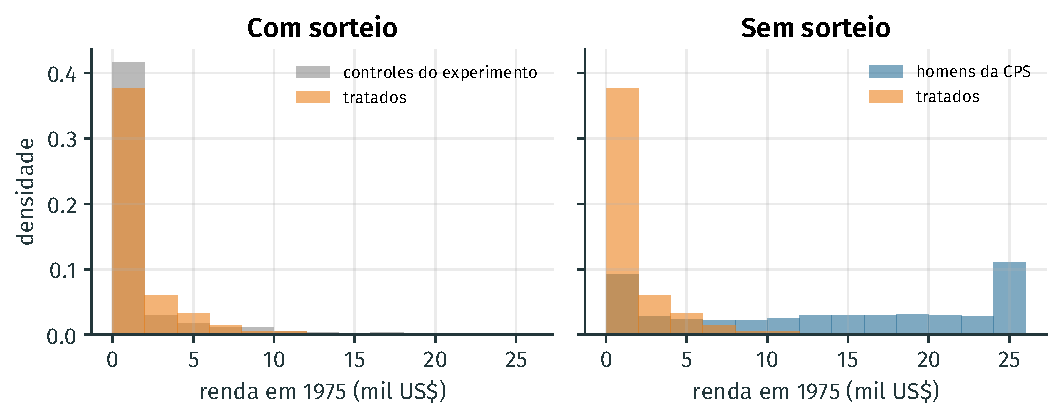
\includegraphics[width=\linewidth]{a02_nsw_re75}
  \caption{Renda em 1975, antes do programa. À esquerda, tratados e controles do
  experimento têm distribuições quase iguais. À direita, os homens da CPS
  ganhavam muito mais; a pilha em US\$ 25 mil é o teto da pesquisa, que não
  divulga rendas acima dele.}
  \label{fig:a02-re75}
\end{figure}

Controlar pelas covariáveis numa regressão ajuda muito, mas não resolve: o
coeficiente do tratamento vai a US\$ 699, ainda longe dos US\$ 1.794 do
experimento (\cref{tab:a02-efeitos}). A regressão linear impõe uma forma
funcional e extrapola para regiões em que quase não há tratados, como a de
rendas altas. Na Aula~6 voltaremos a esse problema com ferramentas de
aprendizado de máquina.

\begin{table}[ht]
  \centering\small
  \caption{Efeito do NSW sobre a renda de 1978 segundo diferentes comparações.}
  \label{tab:a02-efeitos}
  \begin{tabular}{@{}lr@{}}
    \toprule
    Comparação & Efeito estimado (US\$) \\
    \midrule
    Experimento: diferença de médias            & 1.794 \\
    Experimento: MQO com covariáveis            & 1.676 \\
    Tratados $\times$ CPS: diferença de médias  & $-$8.498 \\
    Tratados $\times$ CPS: MQO com covariáveis  & 699 \\
    \bottomrule
  \end{tabular}
\end{table}

\section{JAX: derivadas e gradiente descendente}

O MQO tem fórmula fechada, mas a maior parte dos modelos de aprendizado de
máquina não tem. Eles são treinados descendo a função de perda passo a passo, e
para isso é preciso calcular derivadas. O \pkg{JAX} tem a mesma interface do
\pkg{NumPy} e acrescenta \py{jax.grad}, que recebe uma função escrita em Python
e devolve a função derivada, calculada de forma exata por diferenciação
automática \parencite{baydin2018}.

A derivada aponta para onde a função sobe. Andando um pouco no sentido
contrário, ela desce. Para um vetor de parâmetros $\vtheta$ e uma perda
$\loss$, a regra do \emph{gradiente descendente} é
\begin{equation}\label{eq:a02-gd}
  \vtheta \leftarrow \vtheta - \lr\,\nabla_{\vtheta}\loss(\vtheta),
\end{equation}
em que $\lr$ é a \emph{taxa de aprendizado}, o tamanho do passo. No notebook,
$\loss$ é o erro quadrático médio do modelo $\widehat{re78} = a + b\cdot treat$
(renda em mil US\$), e o treino inteiro cabe em poucas linhas:

\begin{codigo}
import jax, jax.numpy as jnp
def eqm(params):
    a, b = params
    return jnp.mean((y - a - b * t) ** 2)

grad_eqm = jax.grad(eqm)
params = jnp.array([0.0, 0.0])
for _ in range(60):
    params = params - 0.5 * grad_eqm(params)
# params ~ [4.555, 1.794]: o mesmo resultado do MQO
\end{codigo}

\begin{conexao}
O gradiente do EQM é, a menos do fator $-2/n$, o lado esquerdo das condições
de primeira ordem da \cref{eq:a02-cpo}. O gradiente descendente para quando o
gradiente zera, isto é, exatamente na solução de MQO. Para a regressão linear,
ele é um caminho mais longo para o mesmo lugar; para modelos sem fórmula
fechada, é o único caminho.
\end{conexao}

O tamanho do passo importa (\cref{fig:a02-gd}). Com $\lr = 0{,}1$ o EQM cai
devagar; com $\lr = 0{,}5$ converge em poucos passos; com $\lr = 1$ o passo é
grande demais, os parâmetros ``pulam'' o vale e o EQM explode. Escolher o passo,
e preparar os dados para que um bom passo exista, é tema da Aula~4.

\begin{figure}[ht]
  \centering
  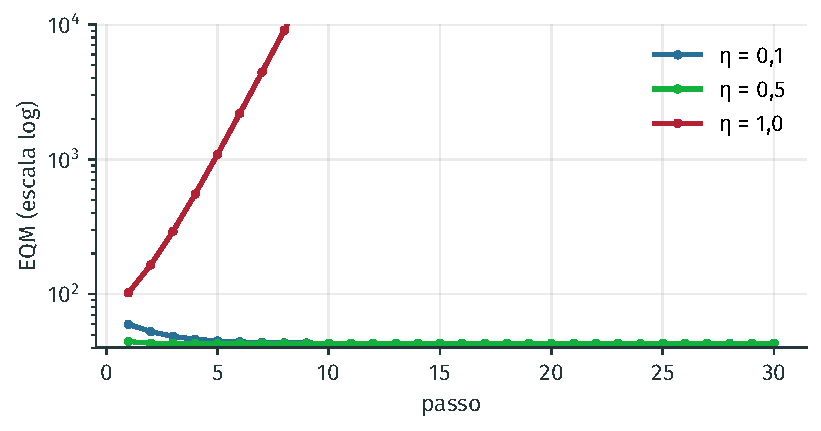
\includegraphics[width=0.72\linewidth]{a02_gd_eta}
  \caption{Erro quadrático médio ao longo do treino por gradiente descendente,
  para três taxas de aprendizado.}
  \label{fig:a02-gd}
\end{figure}

\section{scikit-learn: modelos prontos}

Todo modelo do \pkg{scikit-learn} \parencite{pedregosa2011} segue o mesmo
roteiro: criar o modelo, \py{fit} nos dados de treino e \py{predict} em dados
novos. Essa uniformidade permite trocar de modelo mudando uma linha.

\subsection{Prever a renda}

Na CPS, separamos 30\% dos homens para teste e treinamos modelos para prever a
renda de 1978 a partir das covariáveis. Prevendo a média para todos, o erro
típico (RMSE) no teste é de 9,55 mil dólares; a regressão linear o reduz para
6,93 mil, e uma floresta aleatória chega a 6,95 mil, um empate. Dois fatos
explicam o resultado. A renda de 1975 sozinha carrega quase toda a informação
útil, e a relação com ela é aproximadamente linear. Além disso, as pilhas de
rendas iguais a zero e no teto da pesquisa limitam o que qualquer modelo
consegue prever.

\begin{atencao}
O modelo mais sofisticado nem sempre vence. Compare sempre com uma referência
ingênua (a média) e com a regressão linear. E lembre que coeficientes e
``importâncias'' de modelos preditivos descrevem padrões úteis para prever, não
efeitos causais.
\end{atencao}

\subsection{Dá para prever quem foi tratado?}

Um uso de aprendizado de máquina muito valioso em avaliação de políticas é o
diagnóstico: se, olhando só para as covariáveis, um modelo consegue adivinhar
quem foi tratado, os grupos não são comparáveis. A regressão logística prevê a
probabilidade de ser tratado, a mesma ideia do \emph{escore de propensão}
\parencite{dehejia1999}.

No experimento, o modelo não separa os grupos: no conjunto de teste do notebook,
a probabilidade média prevista é 0,43 entre os tratados e 0,42 entre os controles.
É o sorteio funcionando. Na comparação com a CPS, ele separa com facilidade:
0,27 entre os tratados e 0,01 entre os homens da CPS (\cref{fig:a02-logit}).
O diagnóstico confirma o viés da seção anterior e sugere um caminho de correção:
comparar os tratados apenas com quem tem probabilidade parecida de ser tratado.
O Exercício~6 da lista explora essa ideia.

\begin{figure}[ht]
  \centering
  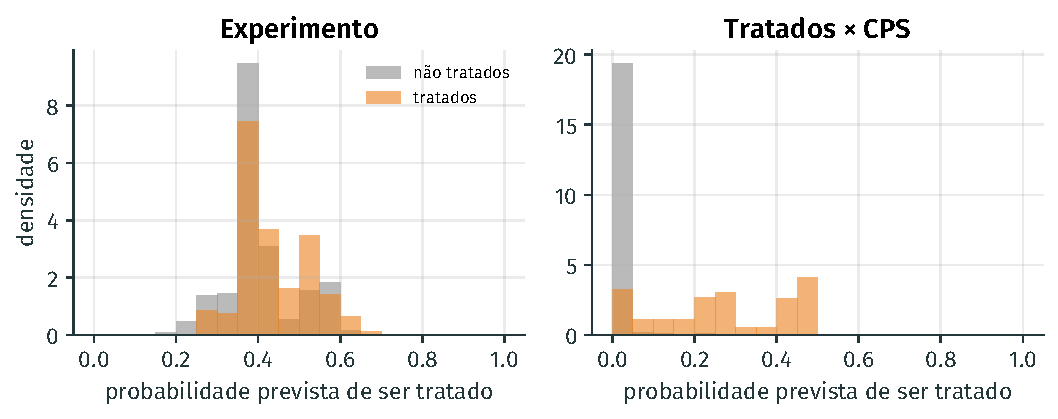
\includegraphics[width=\linewidth]{a02_logit_tratado}
  \caption{Probabilidade prevista de ser tratado por um logit nas covariáveis
  (ajustado na amostra inteira). No experimento, as distribuições se sobrepõem;
  na comparação com a CPS, quase todos os não tratados têm probabilidade perto
  de zero.}
  \label{fig:a02-logit}
\end{figure}

\section{Resumo e leituras}

\begin{itemize}[nosep]
  \item Python oferece os blocos básicos: tipos, listas, dicionários,
        condicionais, laços e funções.
  \item O \pkg{NumPy} substitui laços por operações vetorizadas e traz a álgebra
        matricial; o MQO cabe em uma linha.
  \item O \pkg{pandas} lê, filtra, agrupa e empilha bases de dados.
  \item Com sorteio, a diferença de médias, que é o coeficiente de uma
        \emph{dummy} no MQO, estima o efeito do programa (US\$ 1.794 no NSW).
  \item Sem sorteio, o viés de seleção pode dominar: com a CPS, o sinal inverte.
  \item O gradiente descendente chega ao MQO sem fórmula, se o passo for bem
        escolhido; o \pkg{JAX} calcula os gradientes.
  \item O \pkg{scikit-learn} padroniza o roteiro \py{fit}/\py{predict}; modelos
        preditivos também servem para diagnosticar comparações.
\end{itemize}

\noindent\textbf{Leituras sugeridas.} Para quem está começando a programar,
\textcite[caps.~1--10]{downey2016} e os cursos gratuitos do Kaggle Learn
(\emph{Python}, \emph{Pandas} e \emph{Intro to Machine Learning}). Sobre o
experimento, o artigo original de \textcite{lalonde1986} e a reanálise de
\textcite{dehejia1999}. Sobre arrays, \textcite{harris2020}; sobre
diferenciação automática, \textcite{baydin2018}.

\input{../aulas/03-treino-teste-validacao/conteudo}
\input{../aulas/04-gradiente-descendente/conteudo}
\input{../aulas/05-arvores-redes/conteudo}
\input{../aulas/06-casos-economia/conteudo}

\clearpage
\printbibliography[heading=bibintoc, title={Referências}]
\end{document}
